\documentclass[oneside]{article}

% Font
\usepackage[T1]{fontenc}
\usepackage[utf8]{inputenc}
\usepackage{lmodern}

% For symbols
\usepackage{pifont}
\newcommand{\xmark}{\ding{53}} % x

% For tables
\usepackage{adjustbox}
\usepackage{multirow}
\usepackage{color, colortbl}
\definecolor{Gray}{gray}{0.95}
\usepackage{hhline}

% For identing the table at the right place
\usepackage{float}

% For left spacing
\usepackage{scrextend}

% For images
\usepackage{graphicx}
\usepackage[labelfont=bf]{caption}
\graphicspath{ {./images/} }

% links
\usepackage{hyperref}

% writting code
\usepackage{listings}
\definecolor{dkgreen}{rgb}{0,0.6,0}
\definecolor{gray}{rgb}{0.5,0.5,0.5}
\definecolor{mauve}{rgb}{0.58,0,0.82}
\lstset{frame=tb,
  language=python,
  aboveskip=3mm,
  belowskip=3mm,
  showstringspaces=false,
  columns=flexible,
  basicstyle={\small\ttfamily},
  numbers=none,
  numberstyle=\tiny\color{gray},
  keywordstyle=\color{blue},
  commentstyle=\color{dkgreen},
  stringstyle=\color{mauve},
  breaklines=true,
  breakatwhitespace=true,
  tabsize=3
}

% for shorter paragraph spaces
\setlength{\parindent}{1ex}
\setlength{\parskip}{0.5ex}
% for first paragraphs
\newcommand*\fpar{\hspace{1ex}}
\newcommand*\ccell [1]{\multicolumn{1}{c|}{\textbf{#1}}}
\newcommand*\ccelll[1]{\multicolumn{1}{c }{\textbf{#1}}}

\title{Project - Phase 5 Stress Testing}
\author{Group 14 \\
Tiago Carvalho fc51034 \\
Diogo Lopes fc51058 \\
Miguel Saldanha fc51072 \\
João Roque fc51080 \\
João Afonso fc51111 \\
}
\date{14/04/2021}

% The report is expected to:
  % Document the actual contributions in the various phases
  % Discuss the options taken throughout the project
  % Use diagrams and tables that summarize the ideas and results
  % Point future improvements

%  The report should not:
  % Explain concepts
  % Detail used frameworks, methodologies …
  % Use generic images or diagrams

\begin{document}
\maketitle

\section{Introduction}
\fpar To perform an evaluation on the system by stress testing, we used three different technologies: Prometheus, Grafana and Locust. 
\par Prometheus is a monitoring system that retrieves data directly from the cluster as it is executing, while Grafana displays and amalgamates the data in a way that can be analyzed by the human eye (plots, etc.). 
\par To perform the stress tests on itself, we used Locust, a stress testing tool. 
\par All these tools were configured automatically with scripts to further automate the deployment of the system (see locust.sh and add\_plugins.sh).
\section{Evaluation}
  \fpar We ran Locust, the tool to perform the stress testing, in another cluster to avoid affecting the results. 
  \par It was tested with up to 800 users, which at that point it was getting close to 100\% CPU usage, according to Grafana. At the time, we were using weak machines (12 CPUs) as Google Cloud's free trial did not allow any higher than that. We later got access to better machines and so we tested with up to 6800 users, which was still limited by quotas since we couldn't spawn more users to do so.
  \par Every aspect of the system was being tested: getting entries, putting new entries, get pages from the database, get a recommendation (and even the login and logout which was later changed and so there is no need for load testing as it is handled by an exterior service, auth0). We did stress testing with 100 users, 500 users, 800 users, and later, when we had access to better machines, up to 6800 users.
\section{Validation}
  \fpar With 800 users the system reached around 75\% CPU usage and 2000 to 2500\% system load, which we assume to be a somewhat comfortable limit for the resources we have, it can go higher, but it could probably start running into performance problems after a certain point (images in appendix \ref{appendix}).
  \par The latency remained good nonetheless, around 2 to 4ms. Disk usage was always very low as most of the data was not stored in the cloud but rather on an exterior database (MongoDB and MySQL). There was a high usage of memory though, probably to store all the requests (around 14gb).
  \par When we later tested with 6800 users, we got to around 600\% CPU usage, which is equivalent to 6 CPUs running at their full potential. System load had spikes of up to 400\% and the memory usage was around 35\%. Since most of the load was concentrated on the api-gateway, we increased it's scaling capabilities immensely, with it getting to 100 pods, give or take. As mentioned before, our system could be tested with a bigger load, but unfortunately we were limited by the quotas.
\section{results}
\begin{figure}[H]
  \centering
  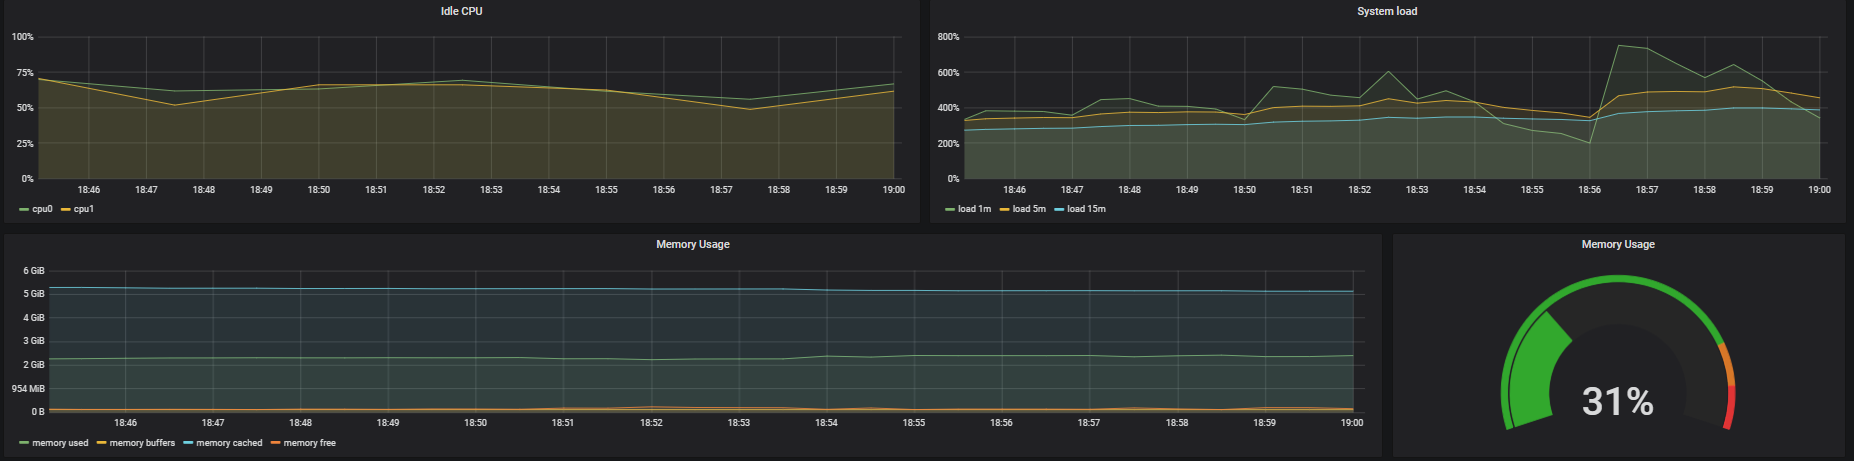
\includegraphics[width=\textwidth]{ img1.png }
  \caption{Stress testing with 800 users. CPU usage and system load plots}
\end{figure}
\begin{figure}[H]
  \centering
  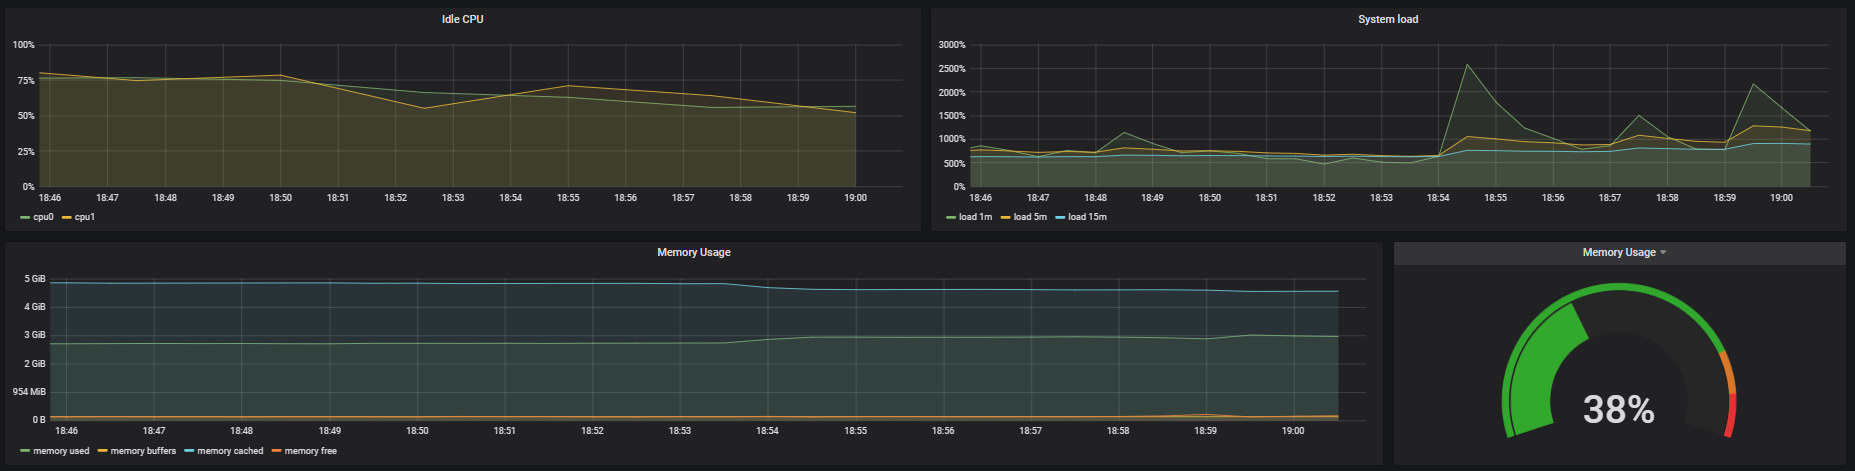
\includegraphics[width=\textwidth]{ img2.png }
  \caption{Stress testing with 800 users. CPU usage and system load plots}
\end{figure}
\begin{figure}[H]
  \centering
  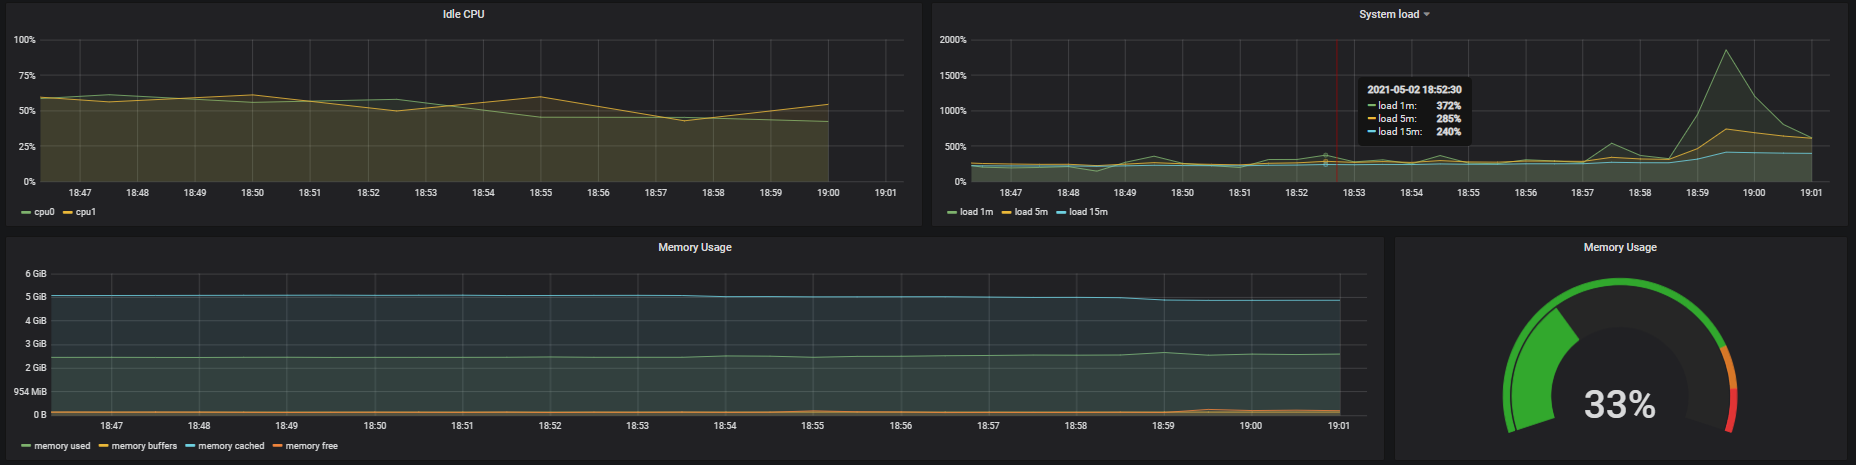
\includegraphics[width=\textwidth]{ img3.png }
  \caption{Stress testing with 800 users. CPU usage and system load plots}
\end{figure}
\begin{figure}[H]
  \centering
  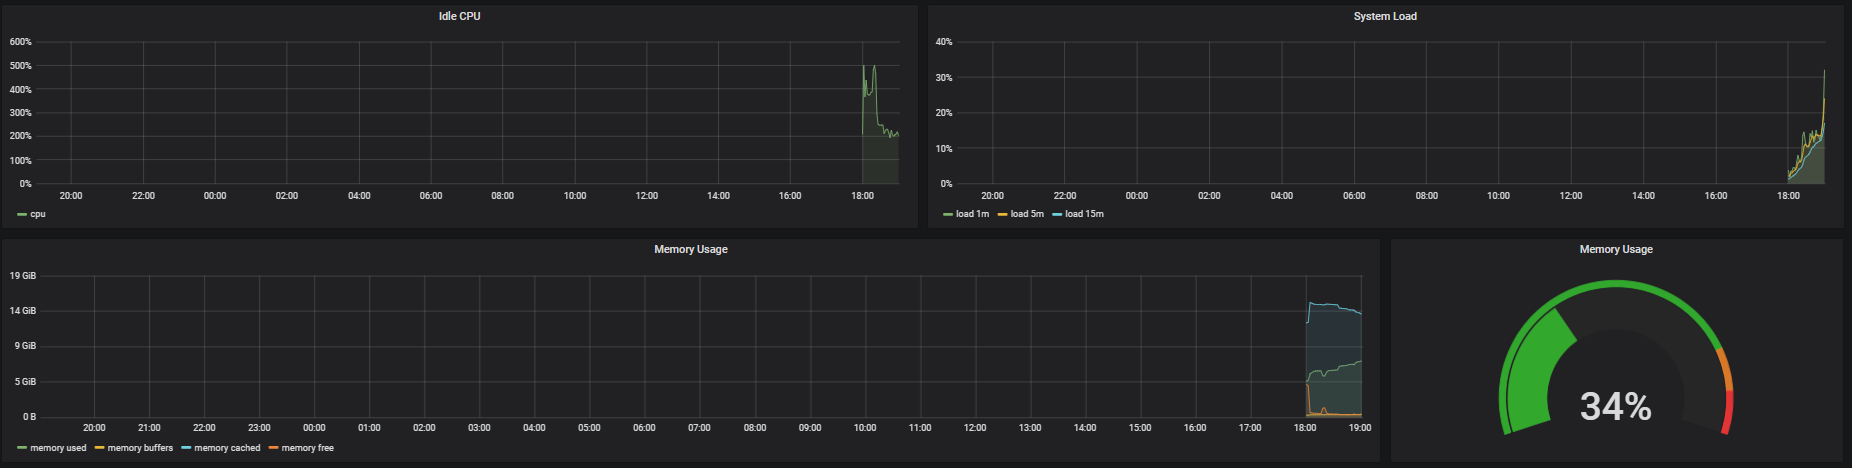
\includegraphics[width=\textwidth]{ img4.png }
  \caption{Stress testing with 800 users. CPU usage and system load plots}
\end{figure}
\begin{figure}[H]
  \centering
  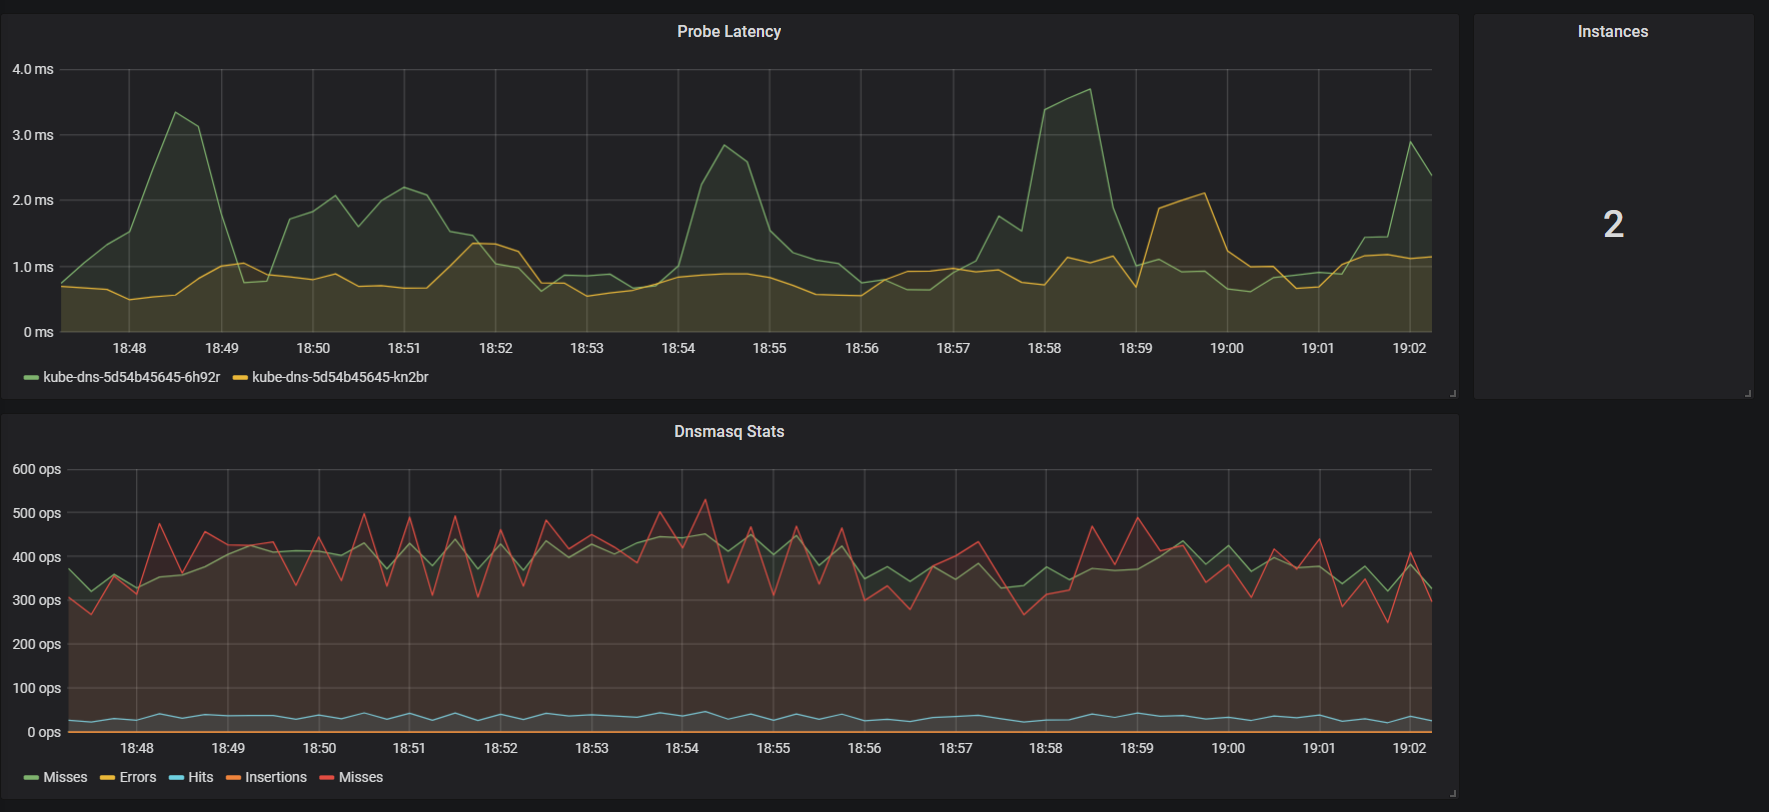
\includegraphics[width=\textwidth]{ img5.png }
  \caption{Stress testing with 800 users. DNS latency}
\end{figure}
\begin{figure}[H]
  \centering
  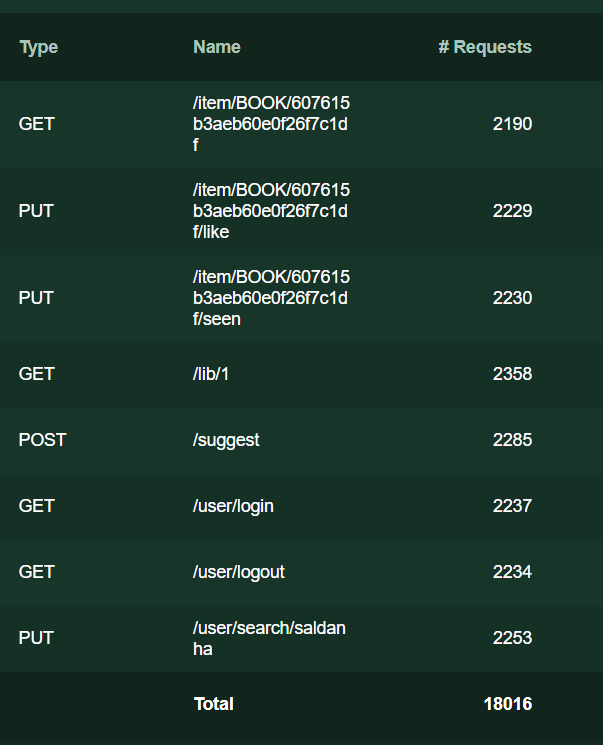
\includegraphics[width=\textwidth]{ locust.png }
  \caption{Stress testing with 800 users, requests and count of each}
\end{figure}
\begin{figure}[H]
  \centering
  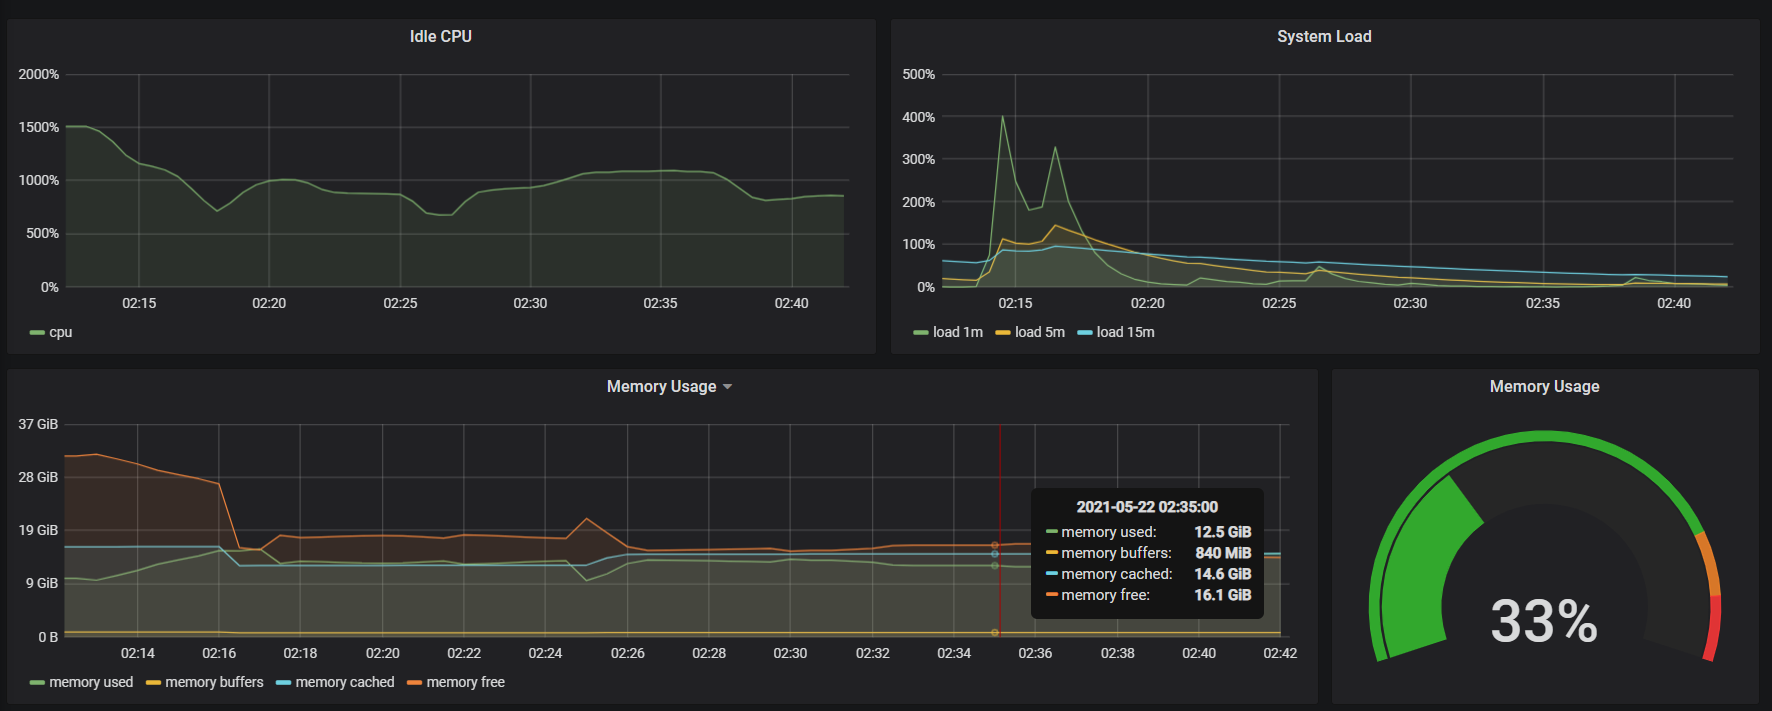
\includegraphics[width=\textwidth]{ 6800.png }
  \caption{Stress testing with 6800 users. Idle CPU and system load plots}
\end{figure}
\begin{figure}[H]
  \centering
  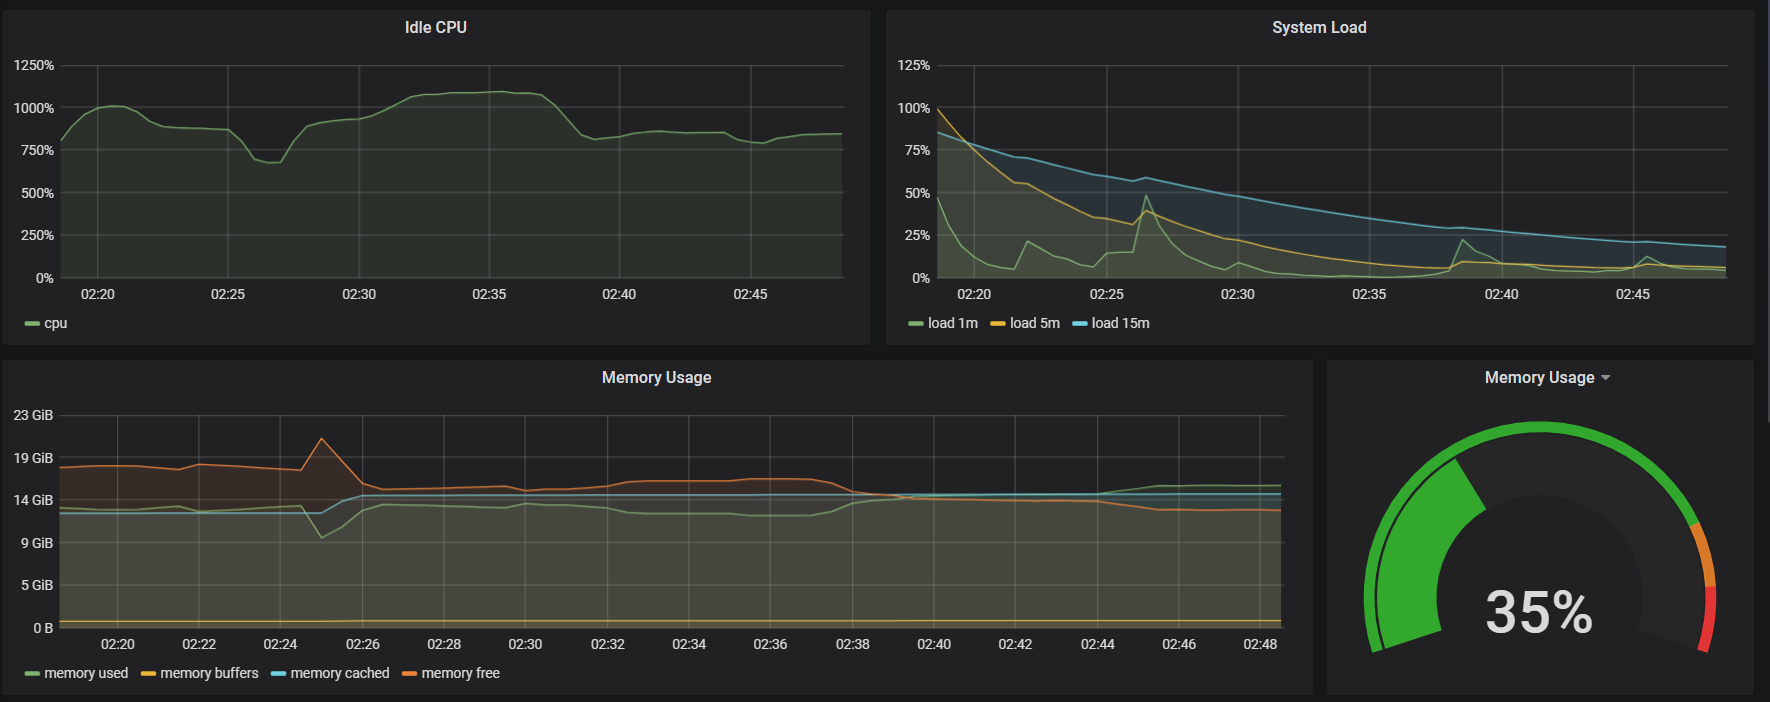
\includegraphics[width=\textwidth]{ 6800stable.png }
  \caption{Stress testing with 6800 users after the system stabilized. Idle CPU and system load plots}
\end{figure}
\end{document}
  

